\chapter{\label{chap:model}Modelo e Implementação}

Conforme visto na seção~\ref{simulator:flow}, um sistema de simulação possui uma
série de componentes conceituais, cada um com suas responsabilidades bem
definidas. Para projetar um simulador, diversas abordagens e paradigmas poderiam
ser aplicadas. Neste estudo optou-se pelo paradigma de \textit{Programação
Orientada a Objetos}. Esta escolha se deu pelos seguintes motivos:

\begin{description}
  \item[Capacidade de Abstração]\hfill \\
    Conceitos da \textit{Programação Orientada a Objetos}, como classes,
    interfaces, polimorfismo, herança e sobrecarga permitem a realização de uma
    modelagem conceitual em alto nível de abstração, permitindo uma explanação
    de fácil entendimento sem ser necessário abordar questões da implementação
    em si (linguagem de programação, arquitetura, etc).
  \item[Padrão de Mercado]\hfill \\
    Desde meados dos anos 90, a \textit{Programação Orientada a Objetos}
    tornou-se frequentemente utilizada no mercado de desenvolvimento de software
    e nos ambientes acadêmicos relacionados à computação. Assim, é possível
    atingir uma maior audiência.
  \item[Domínio dos Autores]\hfill \\
    O paradigma é de domínio dos autores deste estudo.
  \item[Suporte nativo no \texttt{C++}]\hfill \\
    O paradigma é suportado de forma no \texttt{C++11}, linguagem escolhida para
    a implementação.
\end{description}

Nas próximas seções serão apresentados os modelos e detalhes de implementação do
simulador de elevadores.

\textbf{Atenção: algumas simplificações foram realizadas nos modelos UML a fim
de permitir uma melhor compreensão~-~por exemplo, omissão de métodos
\textit{getters} e \textit{setters}.}

\section{\label{model:scenario}Cenário}

Como entrada o simulador recebe um conjunto de cenários e realiza a simulação de
cada um deles. Um cenário é composto pelas seguintes informações:

\begin{description}[leftmargin=!,labelwidth=\widthof{\bfseries Função de Custo}]
  \item[Nome]

  Identificação textual do cenário.

  \item[Duração]

  Tempo durante o qual serão geradas chegadas de clientes aos andares do prédio.
  Após este tempo, não chegarão mais clientes. Porém, clientes que já entraram
  no prédio e estão distribuídos nos andares e elevadores precisam terminar suas
  viagens antes que a simulação chegue ao fim. Devido a isto, é normal que o
  tempo real de simulação seja maior que a duração estipulada no cenário.

  \item[Agendamento]

  Lista de algoritmos de agendamento.

  \item[Horizonte]

  Horizonte de expansão do agendamento com algoritmo de \textit{planning} (não utilizado no agendamento \textit{simple}).

  \item[Função de Custo]

  Lista de funções de custo.

  \item[Semente]

  Semente textual para inicialização os geradores de números aleatórias.

  \item[Elevadores]

  Número de elevatores do prédio.

  \item[Capacidade]

  Capacidade dos elevadores (a mesma para cada elevador).

  \item[Andares]

  Lista com o intervalo médio\footnote{O valor médio informado é utilizado como
  parâmetro $\lambda$ de entrada para uma Distribuição de Poisson. Cada andar do
  prédio possui uma distribuição distinta.} de chegada de passageiros, em
  segundos, para cada andar. A lista começa com a média do andar térreo e segue
  sucessivamente. O número de andares é igual ao tamanho da lista.

\end{description}

Convém salientar que, definido um cenário, será realizada uma simulação para cada
combinação possível de algoritmo de agendamento com função de custo. Por
exemplo, se forem especificados os algoritmos de agendamento \textit{simple} e
\textit{planning} juntamente das funções de custo \textit{nearest neighbour} e
\textit{weighted}, serão realizadas 4 simulações deste cenário com as seguintes
combinações:

\begin{itemize}
  \item Agendamento \textit{simple} com função de custo \textit{nearest neighbour};
  \item Agendamento \textit{simple} com função de custo \textit{weighted};
  \item Agendamento \textit{planning} com função de custo \textit{nearest neighbour};
  \item Agendamento \textit{planning} com função de custo \textit{weighted}.
\end{itemize}

\subsection{\label{model:scenario:config}Arquivo de Configuração}

A entrada de dados para o simulator se dá através de um arquivo de configuração
chamado \texttt{config.yaml}. Este arquivo obedece o padrão \textit{YAML}, um
formato de serialização de dados legíveis por humanos.

\begin{algorithm}[htb]
  \centering
    \begin{minted}[frame=lines,framesep=2mm,linenos,fontsize=\small]{yaml}
scenarios:
  - name: Scenario 1
    duration: 43200 # 12 hours
    scheduler: [ 0, 1 ] # simple, planning
    planningHorizon: 5
    cost_function: [ 1, 3, 4 ] # randon, bnn, weighted
    seed: 54TH7hboAG1iOsDIDhJp
    elevators: 2
    capacity: 6
    floors: [ 60, 520, 360, 240, 240, 90, 90, 90 ]

  - name: Scenario 2
    # ...

  - name: Scenario N
    # ...
    \end{minted}
  \caption{Exemplo de arquivo de configuração \texttt{config.yaml}.}
  \label{alg:config}
\end{algorithm}

No exemplo do algoritmo~\ref{alg:config} são definidos alguns cenários. No
primeiro, chamado \texttt{Scenario 1}, clientes chegarão durante 12 horas
distribuídos ao longo dos 8 andares do prédio e serão atendidos por um dos 2
elevadores, cuja capacidade é de 8 passageiros cada. Pode ser definido um
número ilimitado de cenários no arquivo de entrada.

Para representar as informações referentes a um cenário foi criada a classe
\texttt{Scenario} (figura~\ref{fig:diagram:scenario}). Além de armazenar as
informações, disponibiliza o método \texttt{Load}, cujo objetivo é carregar os
cenários a partir do arquivo de configuração utilizando a biblioteca \texttt
{yaml-cpp}.

\begin{figure}[htb!]
  \centering
  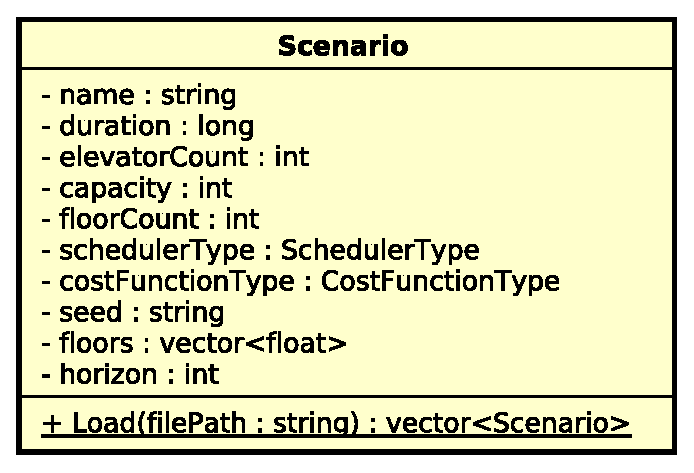
\includegraphics[scale=0.6]{img/Scenario}
  \caption{Diagrama de classes dos \textit{cenários}.}
\label{fig:diagram:scenario}
\end{figure}

\section{\label{model:events}Eventos}

A simulação de eventos discretos, como o próprio nome já diz, é orientada a
eventos. Isso significa dizer que as alterações no estado do sistema ocorrerão
somente na ocasião de algum evento e é preciso ser possível representar um
evento no contexto do simulador. Um evento é uma estrutura que deve possuir as
seguintes informações: (1) um número identificador; (2) o horário agendado para
a ocorrência do evento; (3) o tipo do evento.

Existem dois tipos de eventos que podem ocorrer durante uma simulação:

\begin{description}
  \item[Chegada de cliente] Um cliente chegou na fila de um andar.

  \item[Fim da simulação] A simulação atingiu a duração
especificada.\footnote{Este evento não necessariamente implica no fim imediato
da simulação, apenas que a chegada de novos clientes não ocorrerá mais. O
simulador ainda irá processar os clientes que estiverem nos andares ou dentro de
elevadores.}

\end{description}

Para obter tal funcionalidade foram criadas a classe abstrata \texttt{Event} e
as classes concretas que a especializam, representando os eventos de
\textbf{chegada de cliente} e \textbf{fim da simulação}, respectivamente:
\texttt{ClientArrival} e \texttt{FinishSimulation}
(figura~\ref{fig:diagram:events}).

\begin{figure}[htb!]
  \centering
  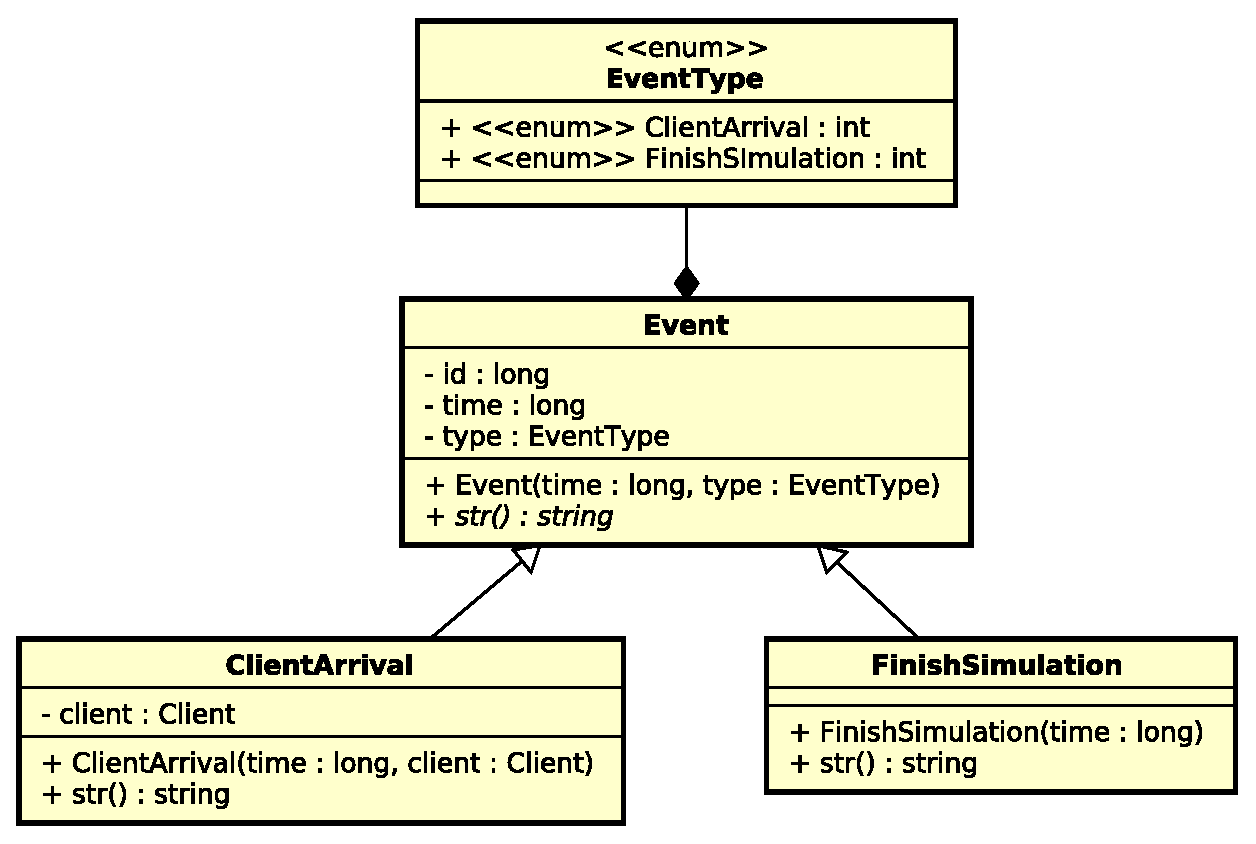
\includegraphics[scale=0.6]{img/Events}
  \caption{Diagrama de classes dos \textit{eventos e seus derivados}.}
\label{fig:diagram:events}
\end{figure}

\begin{description}
  \item[Event] \hfill \\
    Evento base composto pelo conjunto básico de informações para um evento.

    \begin{description}[leftmargin=!,labelwidth=\widthof{\bfseries client}]
      \item[\texttt{id}] Número identificador do evento.
      \item[\texttt{time}] Horário de ocorrência do evento.
      \item[\texttt{type}] Tipo do evento.
    \end{description}

  \item[ClientArrival] \hfill \\
    Evento especializado do tipo \textbf{chegada de cliente}. Contém,
    adicionalmente, as informações do cliente.

    \begin{description}[leftmargin=!,labelwidth=\widthof{\bfseries client}]
      \item[\texttt{client}] Cliente que gerou o evento.\footnote{Tipo complexo armazenando diversas informações sobre o cliente. \unsure{Colocar referência.}}
    \end{description}

  \item[FinishSimulation] \hfill \\
    Evento especializado do tipo \textbf{fim da simulação}. Não é necessária
    nenhuma informação adicional.
\end{description}

\section{\label{sec:model:event}Gerenciamento de eventos}

Na seção~\ref{simulator:flow} foram apresentados os componentes de um simulador.
Alguns destes componentes devem reagir na ocorrência de um evento, alterando o
seu estado interno de acordo com o tipo de evento ocorrido e as informações que
ele carrega consigo. Porém restam as questões de como saber qual evento será o
próximo a ocorrer e como notificar os elementos reativos disso. Portanto,
precisamos de mecanismos para criar e ordenar eventos e notificar os componentes
da ocorrência de um evento.

\subsection{Criação}

Não é possível prever em qual andar e qual momento um cliente irá chegar ao
prédio, tampouco qual o destino desejado por ele. Portanto, é correto afirmar
que a chegada de clientes em um prédio é um processo estocástico.

\subsubsection{Horário de chegada}

Segundo~\cite{Ross:2006:IPM:1197141}, a taxa de chegada de clientes é um
processo de Poisson, com razão $\lambda$. Ou seja, o tempo entre novos clientes
são variáveis independentes, com valor esperado $\frac{1}{\lambda}$. Pode-se ver
na figura~\ref{fig:distribution:poisson} um exemplo de diferentes valores de
$\lambda$ gerando diferentes distribuições.

\begin{figure}[htb!]
  \centering
  \includegraphics[scale=1.0]{img/poisson.eps}
  \caption{Exemplo de distribuições de Poisson.}
\label{fig:distribution:poisson}
\end{figure}

Em um prédio no mundo real, esta distribuição varia de acordo com a hora do dia.
Por exemplo, nos horários do início do turno da manhã e no início do turno da
tarde, muito mais passageiros chegam ao térreo, com destino ao andar onde
trabalham. Para fim de simplificação, esta variação ao longo do dia não foi
considerada neste estudo. Conforme visto na seção \ref{model:scenario}, cada
andar do prédio possui um valor para $\lambda$, que permanece constante no
decorrer de toda a simulação.

\subsubsection{Andar de destino}

Já a probabilidade de um cliente ir de um andar para outro, em um tráfego
chamado de \textit{interfloor}, é um processo de Markov, com distribuições
normais que variam de acordo com a hora do dia.

Uma cadeia de Markov, utilizada para representar este processo, é por sua vez
representada por uma matriz de probabilidades. No caso deste sistema, tem-se uma
função com distribuição normal (\textit{i.e.} uma média e um desvio padrão) que
varia de acordo com o horário do dia, para cada posição desta matriz.

Um exemplo de matriz para um prédio de 3 andares é:

\[
  \begin{bmatrix}
    f_{11} & f_{12} & f_{13} \\
    f_{21} & f_{22} & f_{23} \\
    f_{31} & f_{32} & f_{33}
  \end{bmatrix}
\]

Onde cada valor é uma função $f(t)$, com $t$ sendo o momento do dia e resultando
em um valor de média e um valor de desvio padrão para a distribuição naquele
momento. Cada função descreve a probabilidade de um cliente estar em um andar e
desejar ir para outro. Por exemplo, $f_{31}$ descreve a probabilidade de um
cliente estar no terceiro andar e desejar descer para o primeiro.

Além disto, a diagonal principal (\textit{i.e} $f_{11}$, $f_{22}$ e
$f_{33}$) é sempre zero, já que não faz sentido um cliente desejar ir para o
mesmo andar em que se encontra.

Esta cadeia de Markov pode ser vista na figura~\ref{fig:distribution:markov}.

\begin{figure}[htb!]
  \centering
  \includegraphics[scale=0.6]{img/markov.eps}
  \caption{Exemplo de cadeia de Markov para um prédio de 3 andares.}
\label{fig:distribution:markov}
\end{figure}

A figura~\ref{fig:diagram:generator} mostra o diagrama UML da classe que gera eventos.

\begin{figure}[htb!]
  \centering
  \includegraphics[scale=0.6]{img/EventGenerator.eps}
  \caption{Diagrama de classes do \textit{Sistema de Geração de Eventos}.}
\label{fig:diagram:generator}
\end{figure}

\subsection{Priorização}

Na seção~\ref{simulator:movation:discrete} foi apresentado o \textit{mecanismo
de avanço de tempo para o próximo evento}, onde deve-se verificar, em uma lista
de eventos, qual é o próximo evento a ocorrer. Dado um conjunto de eventos
agendados (ou seja, ainda não ocorridos), o primeiro evento a ocorrer é
justamente o que possui o menor tempo de agendamento. Um tipo abstrato de dados
que serve para este propósito é uma \textit{fila prioritária}, ou
\textit{priority queue}, que funciona de forma similar a filas \textit{FIFO},
com a diferença de que cada elemento armazenado possui uma prioridade associada.
A \textit{fila prioritária}, implementada na classe \texttt{EventQueue}, irá
atender os elementos por ordem de prioridade, da maior para a menor. Ao
considerar que a prioridade de um evento é inversamente proporcional ao instante
em que irá ocorrer - ou seja, quanto menor o tempo do evento maior é a sua
prioridade -, temos uma fila na qual o próximo elemento a ser atendido sempre
será o próximo evento a ocorrer.

\begin{description}
  \item[EventQueue] \hfill \\
    Encapsula uma fila prioritária de eventos. Adicionalmente, utiliza a classe
    \texttt{EventComparator}, que implementa a relação de ordem entre os
    eventos.

    \begin{description}[leftmargin=!,labelwidth=\widthof{\bfseries hasNextEvent}]
      \item[\texttt{push}] Insere um evento na fila.
      \item[\texttt{top}] Recupera o primeiro evento da fila.
      \item[\texttt{pop}] Remove o primeiro evento da fila.
      \item[\texttt{hasNextEvent}] Verifica se a fila possui eventos.
    \end{description}
\end{description}

\begin{figure}[htb!]
  \centering
  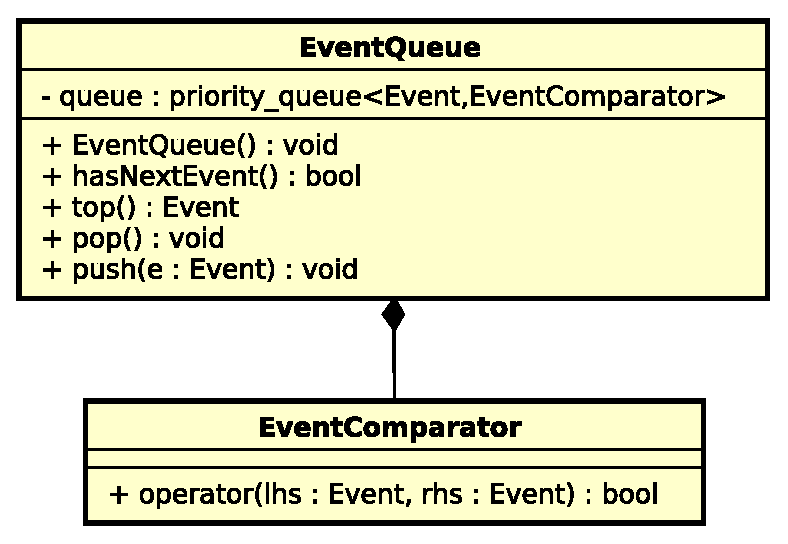
\includegraphics[scale=0.6]{img/EventQueue}
  \caption{Diagrama de classes da \textit{criação e priorização de eventos}.}
\label{fig:diagram:event:manage}
\end{figure}

\subsection{Notificação}

Quando o próximo evento a ocorrer é conhecido, o problema passa a ser notificar
os elementos reativos que este evento ocorreu para que os mesmos possam
atualizar seus estados internos. De acordo com Gamma
\cite{Gamma:1995:DPE:186897}, o padrão \textit{Observer} é um \textit{design
pattern} indicado para resolver este problema. Este \textit{pattern} define uma
dependência de um-para-muitos ($1:N$) entre objetos de modo que, quando este um
objeto (\textit{subject}) tem seu estado alterado, todos os seus dependentes
(\textit{observers}) são notificados deste mudança. Por consequência, estes
dependentes podem modificar seu estado interno baseando-se nas informações desta
notificação.

Este padrão foi utilizado para implementar a funcionalidade de notificação de
eventos, ilustrado no diagrama da figura~\ref{fig:diagram:notification}. Para
isto, foram criados os seguintes componentes:

\begin{figure}[htb!]
  \centering
  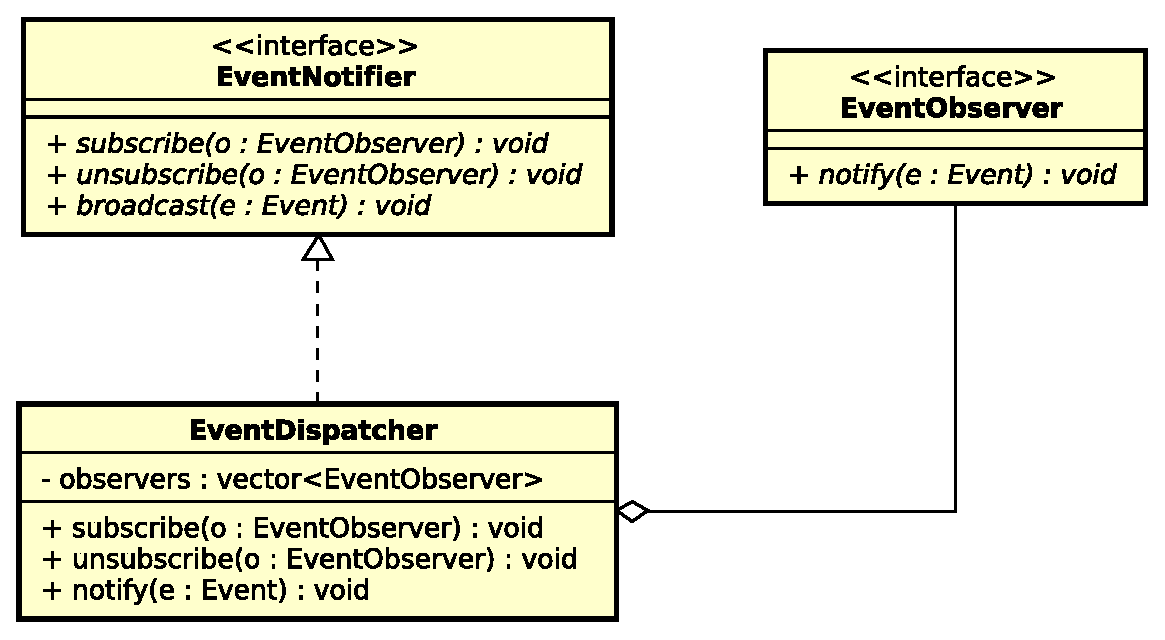
\includegraphics[scale=0.6]{img/EventNotifier}
  \caption{Diagrama de classes da \textit{notificação de eventos}.}
\label{fig:diagram:notification}
\end{figure}

\begin{description}
  \item[EventObserver] \hfill \\
    Classe abstrata a ser realizada por qualquer outra classe que deseje receber
    notificações de eventos. Possui um único método abstrato.

    \begin{description}[leftmargin=!,labelwidth=\widthof{\bfseries unsubscribe}]
      \item[\texttt{notify}] Recebe a notificação da ocorrência de um evento.
    \end{description}

  \item[EventNotifier] \hfill \\
    Classe abstrata a ser realizada por qualquer outra classe que deseje
    notificar a ocorrência de eventos. Define métodos para que objetos que
    implementem a classe abstrata \textit{EventObserver} possam registrar-se
    para receber notificações de ocorrências de eventos. Seus métodos abstratos
    são:

    \begin{description}[leftmargin=!,labelwidth=\widthof{\bfseries unsubscribe}]
      \item[\texttt{subscribe}] Adiciona um \textit{observer}.
      \item[\texttt{unsubscribe}] Remove um \textit{observer}.
      \item[\texttt{broadcast}] Notifica todos os \textit{observers} registrados da ocorrência de um evento.
    \end{description}

  \item[EventDispatcher] \hfill \\
    Classe concreta que realiza a interface \texttt{EventNotifier}. Possui uma
    estrutura de dados para armazenar quais \textit{observers} se registraram
    através dos métodos \texttt{subscribe} e \texttt{unsubscribe}.
\end{description}

Três importantes componentes do simulador podem se beneficiar desta construção:
(1) o \textit{relógio do sistema} (classe \texttt{Clock}); (2) os
\textit{contadores estatísticos} (classe \texttt{Statistics}); e (3) o
\textit{estado do sistema} (classe \texttt{Building}). Na ocorrência de um
evento, estas três entidades devem ser notificadas e cada uma irá alterar seu
estado interno da forma adequada. Para isto, devem implementar a interface
\texttt{EventObserver} e registrarem-se no \texttt{EventDispatcher}. Assim, o
\texttt{EventDispatcher} e a \texttt{EventQueue} podem, juntos, notificar aos
componentes reativos exatamente qual evento ocorreu em cada iteração da
simulação, na ordem correta dos eventos.

\section{\label{model:reactive}Componentes reativos}

Durante a execução da simulação, à medida que eventos ocorrem, componentes do
simulador devem alterar seu estado interno de acordo com o evento ocorrido,
levando o estado do simulador a uma nova situação. A seguir são apresentadas as
classes que representam estes componentes no simulador.

\subsection{Estado do sistema}

Entre os componentes fundamentais de um simulador destaca-se a representação do
\textit{estado do sistema}, uma coleção de variáveis necessárias para descrever
o sistema em um instante em particular da simulação~\cite{Law}. Neste projeto, a
classe \texttt{Building} é responsável por encapsular o conjunto de informações
que definem este estado (figura~\ref{fig:diagram:model}). Esta classe é
responsável por gerenciar múltiplas instâncias de elevadores (classe
\texttt{Elevator}), andares (classe \texttt{Floor}) e clientes (classe
\texttt{Client}) e relacionar estas instâncias entre si - reproduzindo, deste
modo, as dinâmicas do sistema do mundo real que está sendo simulado.

\begin{figure}[htb!]
  \centering
  \includegraphics[scale=0.6]{img/Model.eps}
  \caption{Diagrama de classes do \textit{estado do sistema}.}
\label{fig:diagram:model}
\end{figure}

\begin{description}
  \item[Floor] \hfill \\
    Parte componente de um prédio. Possui os seguintes atributos:

  \begin{description}[leftmargin=!,labelwidth=\widthof{\bfseries arrivalFloor}]
    \item[\texttt{number}] Número do andar em que a parada deve ser realizada.
    \item[\texttt{lambda}] Direção na qual a parada deve ser realizada.
    \item[\texttt{upLine}] Direção na qual a parada deve ser realizada.
    \item[\texttt{downLine}] Direção na qual a parada deve ser realizada.
    \item[\texttt{eventFactory}] Direção na qual a parada deve ser realizada.
  \end{description}

     possuindo uma numeração e duas
    filas\footnote{No mundo real, apesar de aparentemente as pessoas formarem
    uma fila única, os membros da fila respeitam o sentido de viagem do elevador
    e implicitamente separam-se em duas filas: uma para subir e outra para
    descer.}: uma para clientes que desejam descer e outra para clientes que
    desejam subir.

\item[Call] \hfill \\
  Representa uma parada a ser realizada por algum elevador. É composta pelos seguintes
  atributos:

  \begin{description}[leftmargin=!,labelwidth=\widthof{\bfseries arrivalFloor}]
    \item[\texttt{number}] Número do andar em que a parada deve ser realizada.
    \item[\texttt{direction}] Direção na qual a parada deve ser realizada.
  \end{description}

  Por exemplo, pode existir uma parada no andar 8 para subir; uma parada no andar
  4 para descer; etc.

\item[Elevator] \hfill \\
  Representa um elevador. Possui os seguintes atributos:

  \begin{description}[leftmargin=!,labelwidth=\widthof{\bfseries arrivalFloor}]
    \item[\texttt{number}] Número identificador do elevador.
    \item[\texttt{capacity}] Capacidade máxima do elevador (em número de clientes).
    \item[\texttt{location}] Número do andar no qual o elevador se encontra.
    \item[\texttt{destination}] Chamada destino do elevador (classe \texttt{Call}).
    \item[\texttt{status}] Situação atual do elevador: \textit{moving} (movendo-se) ou \textit{idle} (ocioso).
    \item[\texttt{direction}] Direção na qual o elevador está se movendo (no caso de não estar ocioso).
    \item[\texttt{passengers}] Conjunto com os passageiros que embarcaram no elevador e ainda não desembarcaram.
  \end{description}

\item[Client] \hfill \\
  Representa uma pessoa que chegou a um andar e deseja se dirigir a outro andar.
  Possui os seguintes atributos:

  \begin{description}[leftmargin=!,labelwidth=\widthof{\bfseries arrivalFloor}]
    \item[\texttt{id}] Número identificador do cliente.
    \item[\texttt{destination}] Número do andar ao qual o cliente deseja dirigir-se.
    \item[\texttt{arrivalFloor}] Número do andar no qual o cliente chegou.
    \item[\texttt{createTime}] Horário em que o cliente chegou ao prédio.
    \item[\texttt{pickupTime}] Horário em que o cliente embarcou em um elevador.
  \end{description}

  \item[Building] \hfill \\
    Representa a composição do prédio sendo simulado. Possui um conjunto de
    elevadores, uma lista ordenada de andares e um método \texttt{reset},
    utilizado para a inicialização da simulação. Um prédio é formado por no
    mínimo um elevador e no mínimo um andar\footnote{Isto em termos conceituais;
    porém, não há sentido na existência de um sistema de elevadores em uma
    edificação com somente um andar. De fato, conforme afirmado na
    seção~\ref{section:scenarios}, serão simulados prédios com, no mínimo, 4
    andares.}.

\end{description}

\subsection{Relógio da simulação}

O \textit{relógio da simulação} é representado pela classe \texttt{Clock}
(figura~\ref{fig:diagram:clock}). Esta classe encapsula o atributo privado
\texttt{time} e provê métodos para sua consulta e atualização.

\begin{figure}[htb!]
  \centering
  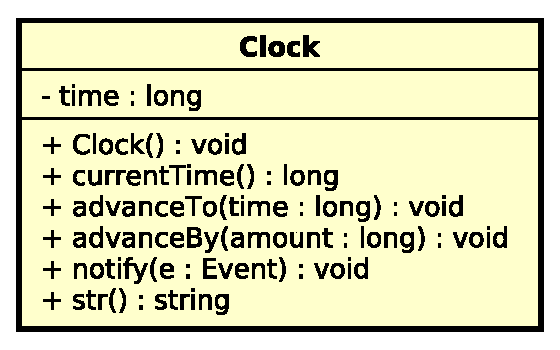
\includegraphics[scale=0.6]{img/Clock}
  \caption{Diagrama de classes do \textit{relógio do sistema}.}
\label{fig:diagram:clock}
\end{figure}

\begin{description}[leftmargin=!,labelwidth=\widthof{\bfseries currentTime}]
  \item[\texttt{currentTime}] Retorna o horário atual do \textit{relógio da simulação}.
  \item[\texttt{advanceTo}] Avança o \textit{relógio da simulação} para um horário arbitrário.
  \item[\texttt{advanceBy}] Avança o \textit{relógio da simulação} em uma quantidade arbitrária de segundos.
  \item[\texttt{str}] Representação textual do \textit{relógio da simulação} (utilizado em \textit{logs}).
  \item[\texttt{notify}]
  Realização da classe abstrata \texttt{EventObserver}. Ao ser notificado de um
  evento, o \textit{relógio da simulação} deve avançar o relógio interno para o
  instante da ocorrência do evento, independentemente do tipo de evento que
  ocorreu. O algoritmo \ref{alg:advanceto} ilustra este conceito.
\end{description}

\begin{algorithm}[htb]
\begin{center}
\begin{algorithmic}[1]
\Function{Clock::Notify}{$event$}
  \State $eventTime \leftarrow event.\Call{getTime}{}$
  \State \Call{advanceTo}{$eventTime$}
\EndFunction
\end{algorithmic}
\end{center}
\caption{\label{alg:advanceto}\textit{Relógio do sistema} reagindo a um evento.}
\end{algorithm}

\subsection{Contadores estatísticos}

Os \textit{contadores estatísticos} da simulação são responsáveis por coletar e
sumarizar dados do sistema durante toda a execução da simulação. Sua existência
permite a realização de análises qualitativas e quantitativas a respeito do
sistema simulado. Neste projeto, os \textit{contadores estatísticos} são
representados pelas estruturas \texttt{Arrival} e \texttt{Trip} e pela classe
\texttt{Statistics} (figura~\ref{fig:diagram:statistics}).

\begin{figure}[htb!]
  \centering
  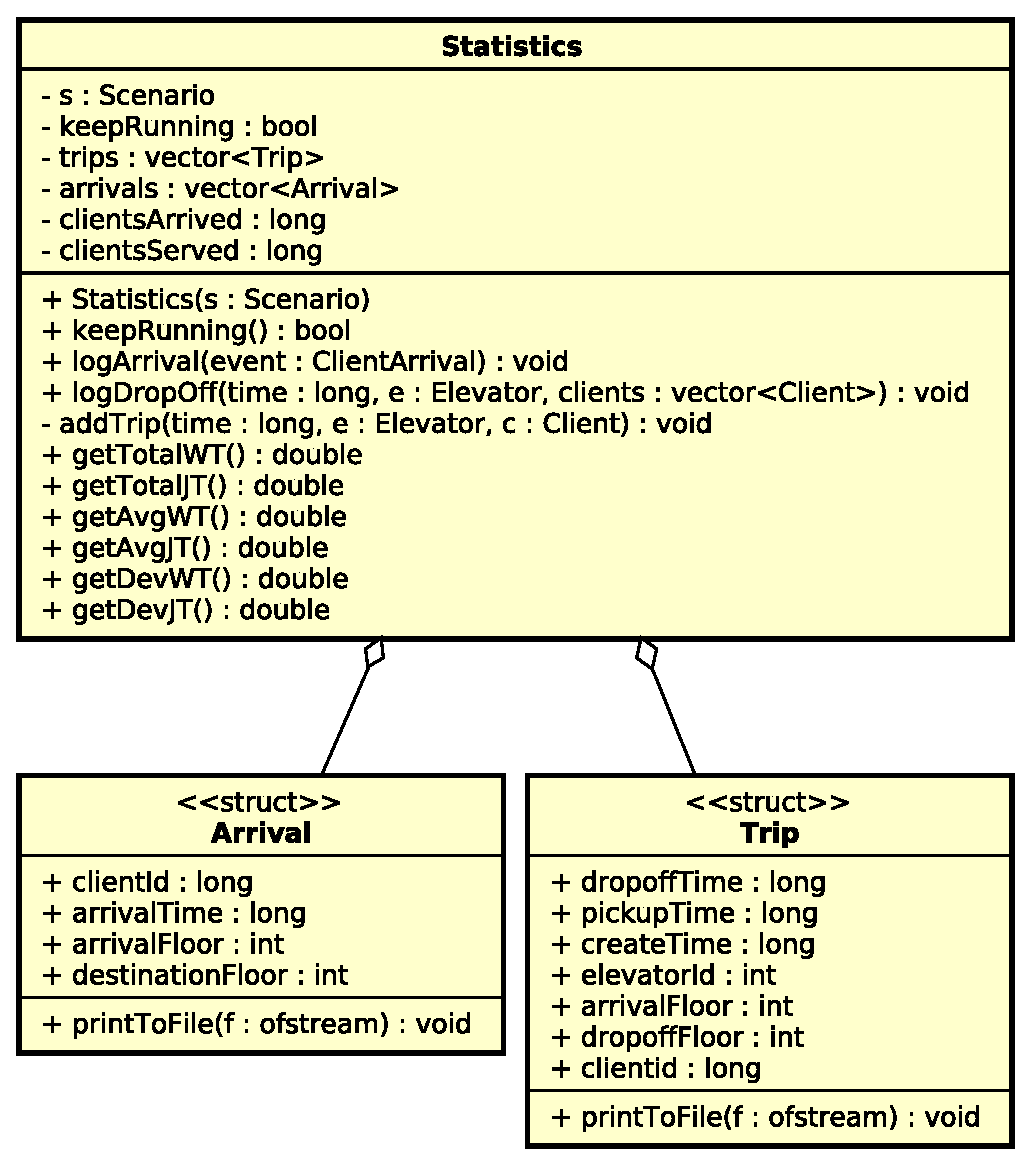
\includegraphics[scale=0.6]{img/Statistics}
  \caption{Diagrama de classes dos \textit{contadores estatísticos}.}
\label{fig:diagram:statistics}
\end{figure}

\begin{description}
  \item[Arrival] \hfill \\
    Uma instância desta estrutura armazena informações coletadas quando um
    cliente chega ao prédio. Tais informações são:

    \begin{description}[leftmargin=!,labelwidth=\widthof{\bfseries destinationFloor}]
      \item[\texttt{clientId}] Número identificador do cliente.
      \item[\texttt{arrivalTime}] Horário em que o cliente chegou ao prédio.
      \item[\texttt{arrivalFloor}] Número do andar no qual o cliente chegou.
      \item[\texttt{destinationFloor}] Andar de destino ao qual o cliente deseja dirigir-se.
    \end{description}

  \item[Trip] \hfill \\
    Uma instância desta estrutura armazena informações coletadas quando um
    cliente desembarca de um elevador. Tais informações são:

    \begin{description}[leftmargin=!,labelwidth=\widthof{\bfseries destinationFloor}]
      \item[\texttt{clientId}] Número identificador do cliente.
      \item[\texttt{dropoffTime}] Horário em que o cliente desembarcou do elevador.
      \item[\texttt{createTime}] Horário em que o cliente chegou ao prédio.
      \item[\texttt{elevatorId}] Número do elevador do qual o cliente desembarcou.
      \item[\texttt{arrivalFloor}] Número do andar no qual o cliente chegou.
      \item[\texttt{dropoffFloor}] Número do andar no qual o cliente desembarcou.
    \end{description}

  \item[Statistics] \hfill \\
    Armazena as estatísticas coletadas durante a simulação e fornece cálculos
    estatísticos sobre o volume de dados coletados no fim da simulação. Seus
    métodos são:

    \begin{description}[leftmargin=!,labelwidth=\widthof{\bfseries destinationFloor}]
      \item[\texttt{logDropOff}] Registra a ocorrência de um desembarque.
      \item[\texttt{logTrip}] Registra a ocorrência de uma chegada de um cliente.
      \item[\texttt{getAvgWT}] Calcula o tempo de espera médio.
      \item[\texttt{getDevWt}] Calculo o desvio padrão do tempo de espera.
      \item[\texttt{getTotalWT}] Calcula o tempo de espera total.
      \item[\texttt{getAvgWT}] Calcula o tempo de jornada médio.
      \item[\texttt{getDevWt}] Calcula o desvio padrão do tempo de jornada.
      \item[\texttt{getTotalWT}] Calcula o tempo de jornada total.
      \item[\texttt{keepRunning}] Avalia se a simulação deve terminar\footnote{por exemplo, se o tempo de duração da simulação já se passou.}.
      \item[\texttt{notify}]
        Realização da classe abstrata \texttt{EventObserver}. Ao ser notificado
        de um evento: se for do tipo \textbf{chegada de cliente}, deve coletar e
        armazenar as informações desta nova chegada; se for do tipo \textbf{fim
        da simulação}, deve altera o estado do atributo privado
        \texttt{keepRunning} para \texttt{false}. Esta ação irá interromper a
        chegada de novos clientes. O algoritmo \ref{alg:statistics} ilustra este
        conceito.
    \end{description}
\end{description}

\begin{algorithm}[htb]
\begin{center}
\begin{algorithmic}[1]
\Function{Statistics::Notify}{$event$}
  \If{$event.$\Call{getType}{} $= ClientArrival$}
    \State \Call{logArrival}{$event$}
  \ElsIf{$event.$\Call{getType}{} $= FinishSimulation$}
    \State $keepRunning \leftarrow false$
  \EndIf
\EndFunction
\end{algorithmic}
\end{center}
\caption{\label{alg:statistics}\textit{Contadores estatísticos} reagindo a um evento.}
\end{algorithm}

  % if (event->getType() == EventType::clientArrival) {
  %   logArrival(std::static_pointer_cast<const ClientArrival>(event));
  % }

  % if (event->getType() == EventType::finishSimulation) {
  %   _keepRunning = false;
  % }

\section{\label{model:simulador}Simulador}

\unsure{Aqui mostrar como o simulador cola todas estas partes e faz funcionar.}

\section{\label{model:schedulers}Algoritmos de Agendamento}
Neste trabalho, dois algoritmos de agendamento foram implementados, o
\textit{Simple Scheduler} (seção~\ref{model:schedulers:simple}) e o
\textit{Planning Scheduler} (seção~\ref{model:schedulers:planning}).

Ambos algoritmos são implementados em classes próprias, que herdam de uma classe
\texttt{Scheduler}. Este relacionamento pode ser visto mais claramente na
figura~\ref{fig:model:schedulers:uml:base}.

\begin{figure}[htb]
  \centering
  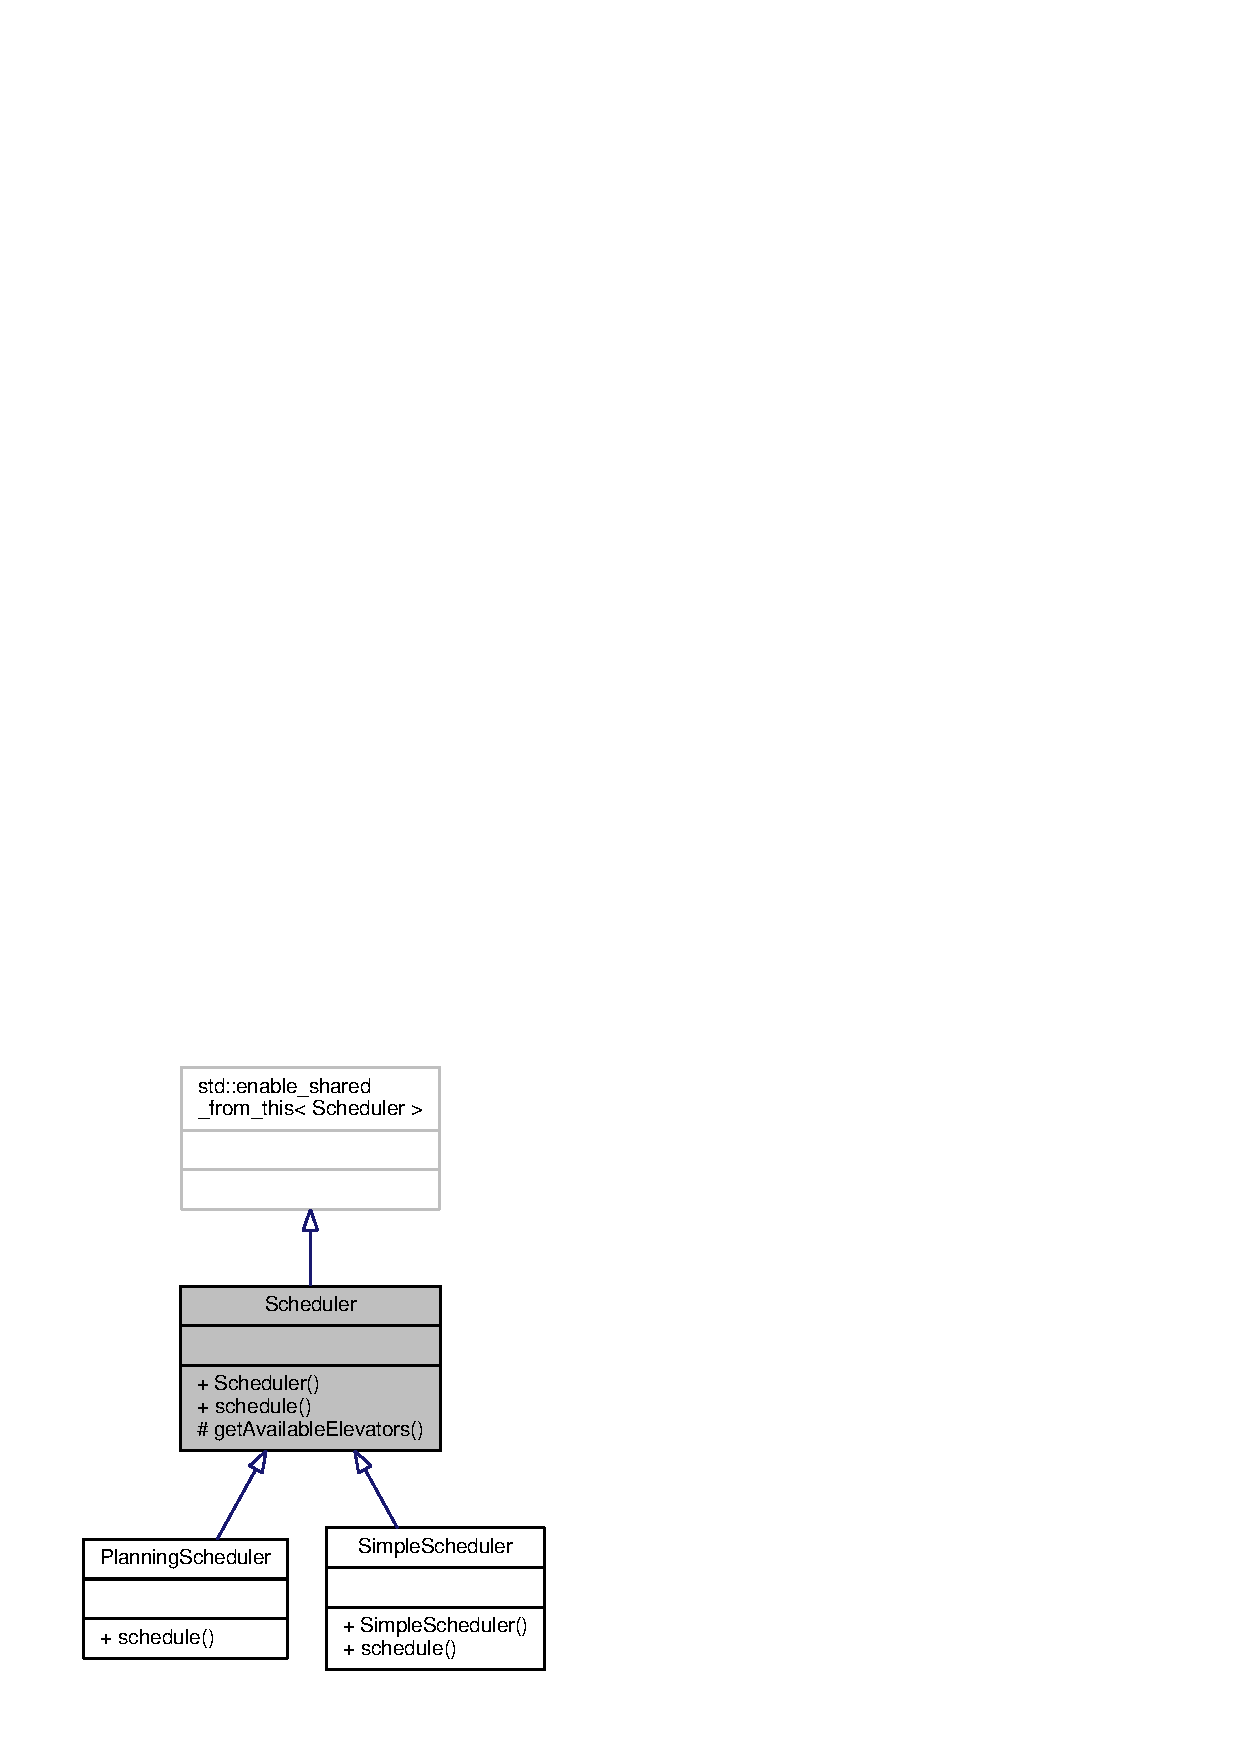
\includegraphics{doc/latex/class_scheduler__inherit__graph}
  \caption{Diagrama UML das classes Scheduler}
  \label{fig:model:schedulers:uml:base}
\end{figure}

Os \textit{schedulers} têm apenas um método público, chamado \texttt{int
  schedule()}, que recebe como parâmetro a função de custo e um ponteiro para o
prédio, além de, opcionalmente, um elevador para ser excluído.

\unsure{Onde falamos de por que é importante excluir elevadores do schedule às
  vezes? (Vanzella)}
Excluir um elevador é importante, como foi falado na Sessão XXX. Há um método
protegido na classe \texttt{Scheduler}, chamado
\texttt{getAvailableElevators()}, que retorna uma lista de elevadores, excluindo
aqueles que não podem ser utilizados.

\subsection{\label{model:schedulers:simple}Simple}
O \textit{Simple Scheduler}, como o nome sugere, tem um comportamento bem
simples: itera pela lista de elevadores disponíveis, calculando a função de
custo para cada um, e retorna o de menor custo.

\subsection{\label{model:schedulers:planning}Planning}
\lipsum[5]

\section{\label{model:costfunctions}Algoritmos de Função de Custo}
As funções de custo herdam de uma classe base, chamada \texttt{CostFunction},
que possui apenas um método público, \texttt{float calculate()}, que retorna o
valor da função para aquela combinação entre o elevador e o cliente.

Isto pode ser visto em mais detalhes na figura~\ref{fig:model:costfunction:uml:base}.

\begin{figure}[htb]
  \centering
  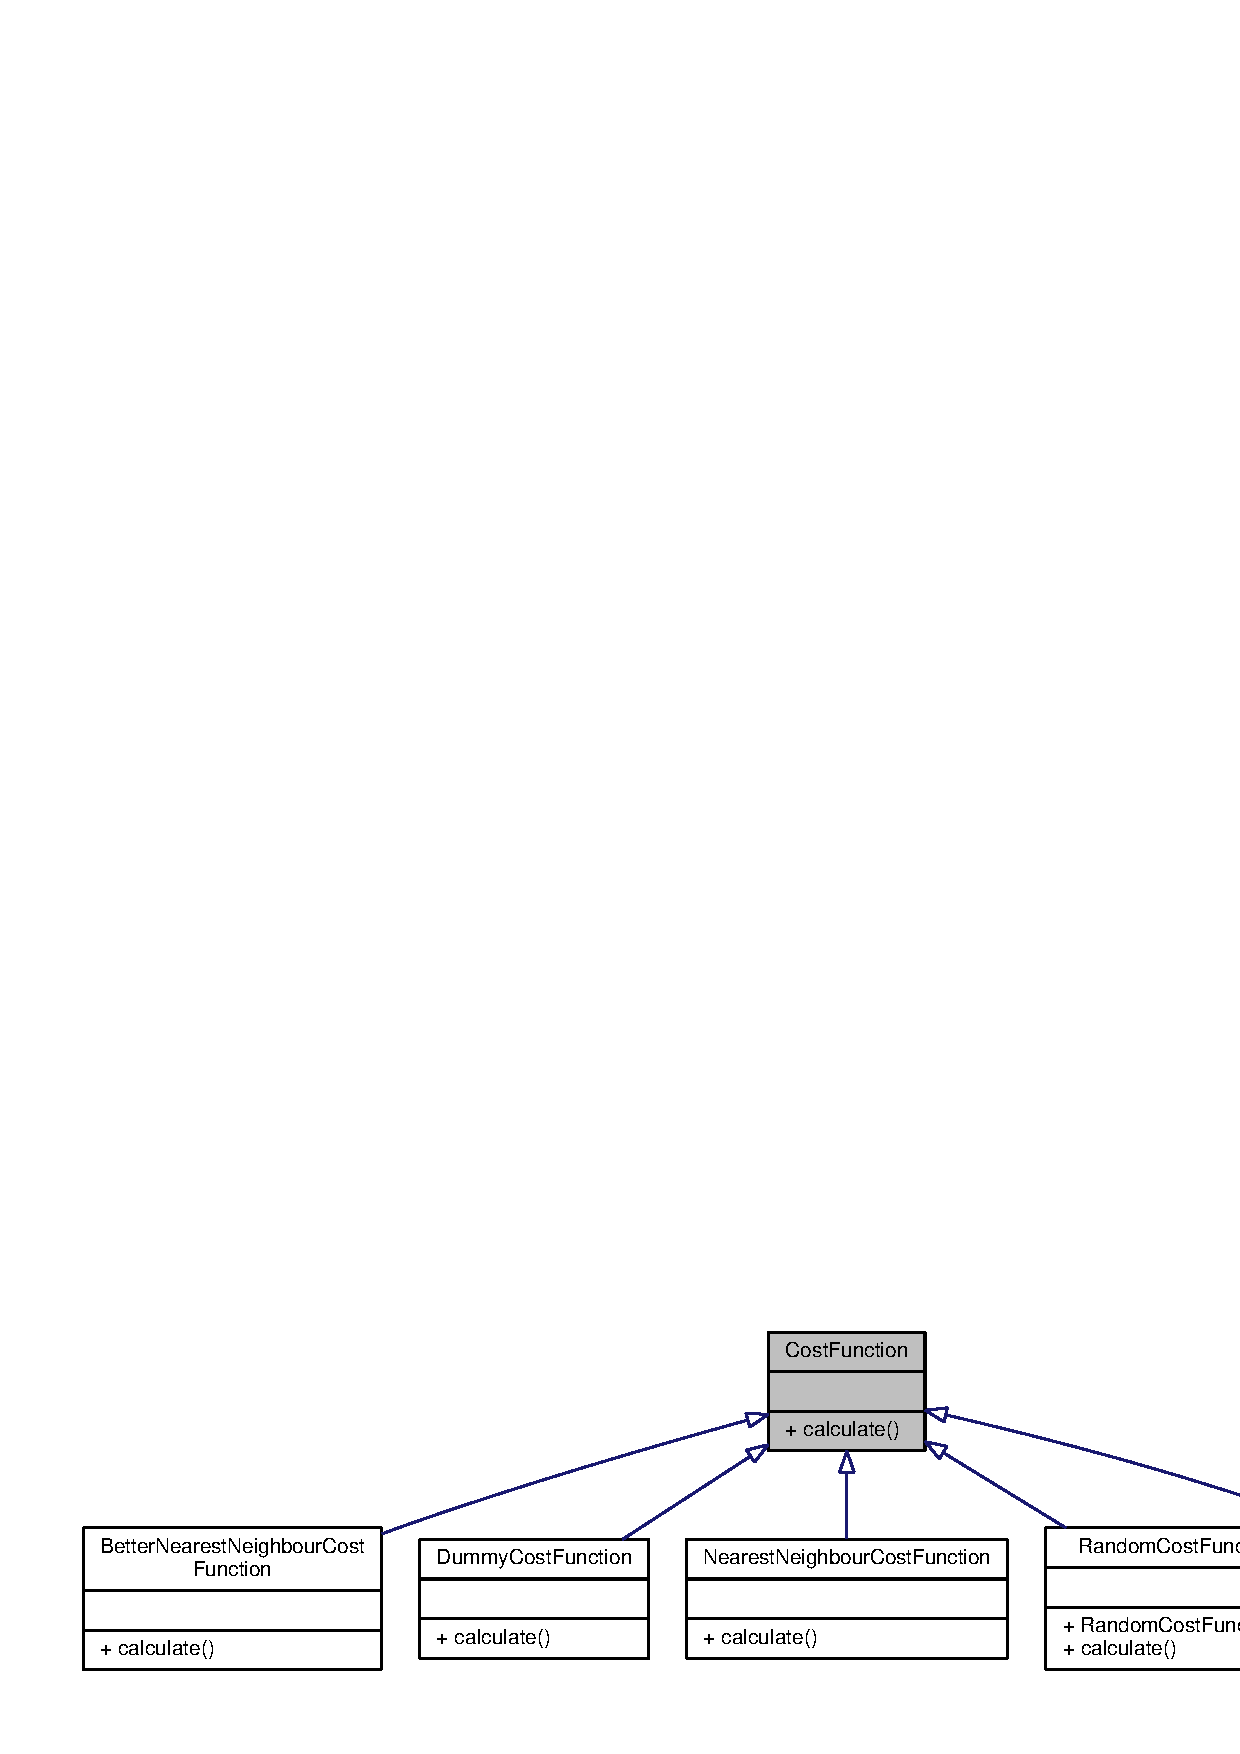
\includegraphics[scale=0.8]{doc/latex/class_cost_function__inherit__graph}
  \caption{Diagrama UML das classes CostFunction}
  \label{fig:model:costfunction:uml:base}
\end{figure}

\subsection{\label{model:costfunctions:random}Random}
A Função de Custo \textit{Random} serve como base de comparação para as demais.
Ela retorna um valor aleatório entre zero e um cada vez que for chamada, e,
portanto, deve resultar em um agendamento pior do que qualquer alternativa.

Olhando-se a figura~\ref{fig:model:costfunction:uml:base}, nota-se que ela é a
única função de custo com um construtor. Isto se dá por que é necessário
inicializar-se a geração de números aleatórios, de modo a gerar estes números de
forma consistente.
\unsure{Vale a pena colocar o código deste construtor aqui? (Vanzella)}

\subsection{\label{model:costfunctions:nn}Nearest Neighbour}
Esta função de custo retorna, como custo, a distância em valor absoluto do
elevador para o cliente. Ela ignora a direção na qual o elevador está viajando.

\unsure{Colocar o código aqui? Tem 2 linhas. (Vanzella)}

\subsection{\label{model:costfunctions:bnn}Better Nearest Neighbour}
A Função de Custo \textit{Better Nearest Neighbour} bonifica elevadores que
estão indo na direção do chamado, dividindo seu custo por $\sqrt 2$ e bonifica
mais ainda os elevadores parados, dividindo seu custo por $2$. O custo antes
deste bônus é calculado de maneira igual à \textit{Nearest Neighbour}.

\subsection{\label{model:costfunctions:weighted}Weighted}
A Função \textit{Weighted} toma uma decisão diferente da \textit{Better Nearest
  Neighbour} para melhorar a \textit{Nearest Neighbour}. Em vez de bonificar
elevadores parados ou elevadores que estão indo na direção do cliente, esta
função bonifica elevadores mais vazios, dividindo o custo (que é a distância
entre o cliente e o elevador) pela ocupação do elevador.\footnote{Como foi visto
na Sessão~XXX, podemos inferir a ocupação pela balança interna do elevador, em
alguns cenários reais.}
\unsure{Sessão XXX (Vanzella)}

\section{\label{model:report}Geração de Relatórios}
\lipsum[5]

\dirtree{%
.1 output.
.2 High-rise\DTcomment{Nome do cenário.}.
.3 1 Simple Random\DTcomment{Diretório da estratégia.}.
.4 run.log\DTcomment{Log de execução da estratégia.}.
.4 report.log\DTcomment{Relatório das métricas da estratégia.}.
.4 trips.log\DTcomment{Arquivo CSV contendo os desembarques.}.
.3 2 Simple NearestNeighbour.
.4 run.log.
.4 report.log.
.4 trips.log.
.3 3 Simple BetterNearestNeighbour.
.4 run.log.
.4 report.log.
.4 trips.log.
.3 4 Simple Weighted.
.4 run.log.
.4 report.log.
.4 trips.log.
.3 5 Planning.
.4 run.log.
.4 report.log.
.4 trips.log.
.3 arrivals.log\DTcomment{Arquivo CSV contendo as chegadas de clientes no prédio.}.
.3 report.log\DTcomment{Relatório unificado de todas as estratégias do cenário.}.
}

\subsection{\label{model:report:charts}Geração de Gráficos}
\lipsum[5]